\psection{Floor Planning}
$$
\left\{\begin{tabular}{c}
    Set of \\ modules
\end{tabular}\right\}
\Rightarrow
\begin{tabular}{l}
- Layout \\
- Network \\
- Pins
\end{tabular}
$$
Optimization goals:
\begin{itemize}
  \item minimize area of global bounding box
  \item minimize total wire length
  \item combination of the above ($\alpha-\beta$)
  \item signal delays (critical path)
\end{itemize}
*Rectangular dissection, division of the chip area into a set of blocks
(non-overlapping rectangles).\\
*Slicing floorplan, rectangular dissection
\begin{itemize}
  \item Obtained by repeatedly dividing each rectangle
  \item Horizontal or vertical cut line
\end{itemize}
*Slicing tree, binary tree with $k$ leaves, $k-1$ internal nodes
\begin{itemize}
  \item Each leaf represents a block
  \item Each internal node represents a h/v cut line
  \item Polish expression ($V \rightarrow *, H \rightarrow +, W \rightarrow \text{wheel}$)
\end{itemize}
\begin{center}
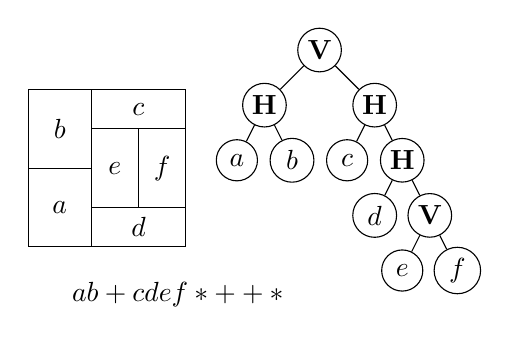
\begin{tikzpicture}
  \begin{scope}
    \draw (0,1) rectangle (0.8,2) node[pos=.5] {$b$};
    \draw (0,0) rectangle (0.8,1) node[pos=.5] {$a$};
    \draw (0.8,0) rectangle (2,0.5) node[pos=.5] {$d$};
    \draw (0.8,1.5) rectangle (2,2) node[pos=.5] {$c$};
    \draw (0.8,0.5) rectangle (1.4,1.5) node[pos=.5] {$e$};
    \draw (1.4,0.5) rectangle (2,1.5) node[pos=.5] {$f$};
  \end{scope}
  \begin{scope}[xshift=3.7cm, yshift=2.5cm,
    every node/.style={draw,circle,
      inner sep=0pt, text width=5mm, align=center
    },
    int/.style={font=\bfseries},
    grow=down,
    sibling distance=14mm,
    level 2/.style={sibling distance=7mm},
    level distance=7mm,
    ]
    \node[int] {V}
      child { node[int] {H}
        edge from parent
        child { node {$a$}
          edge from parent
        }
        child { node {$b$}
          edge from parent
        }
      }
      child { node[int] {H}
        edge from parent
        child { node {$c$}
          edge from parent
        }
        child { node[int] {H}
          edge from parent
          child { node {$d$}
            edge from parent
          }
          child { node[int] {V}
            edge from parent
            child { node {$e$}
              edge from parent
            }
            child { node {$f$}
              edge from parent
            }
          }
        }
      }
    ;
    \begin{scope}[xshift=-1.8cm, yshift=-3.1cm,
      every node/.style={draw=none}]
      \node {$ab+cdef*++*$};
    \end{scope}
  \end{scope}
\end{tikzpicture}
\end{center}
*Non-slicing floorplan (wheels)\\
*Vertical constraint graph (VCG)\\
Edge from node $v_i$ to $v_j$ if block $m_i$ under $m_j$.\\
*Horizontal constraint graph (HCG)\\
Edge from node $v_i$ to $v_j$ \\ if block $m_i$ is left of $m_j$.\\
\vspace{-0.5cm}
\begin{center}
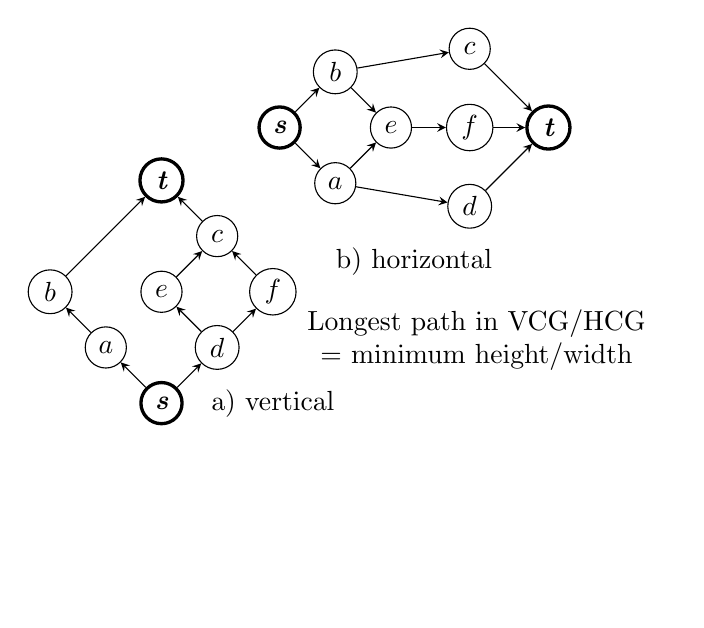
\begin{tikzpicture}[
  >=stealth,
  every node/.style={
    draw,circle,
    inner sep=0pt, text width=5mm, align=center},
  term/.style={font=\bfseries\itshape,very thick},
  lab/.style={draw=none,text width=5cm}]

  \begin{scope}
    \node[term] (s) {s};
    \node[above left of=s] (a) {$a$};
    \node[above left of=a] (b) {$b$};
    \node[above right of=s] (d) {$d$};
    \node[above left of=d] (e) {$e$};
    \node[above right of=d] (f) {$f$};
    \node[above right of=e] (c) {$c$};
    \node[above left of=c,term] (t) {t};

    \draw[->] (s) -- (a);
    \draw[->] (s) -- (d);
    \draw[->] (a) -- (b);
    \draw[->] (d) -- (e);
    \draw[->] (d) -- (f);
    \draw[->] (e) -- (c);
    \draw[->] (f) -- (c);
    \draw[->] (b) -- (t);
    \draw[->] (c) -- (t);

    \node[below right of=d,lab] {a) vertical};
  \end{scope}
  \begin{scope}[xshift=1.5cm, yshift=3.5cm]
    \node[term] (s) {s};
    \node[above right of=s] (b) {$b$};
    \node[below right of=s] (a) {$a$};
    \node[below right of=b] (e) {$e$};
    \node[right of=e] (f) {$f$};
    \node[above of=f] (c) {$c$};
    \node[below of=f] (d) {$d$};
    \node[right of=f, term] (t) {t};

    \draw[->] (s) -- (b);
    \draw[->] (s) -- (a);
    \draw[->] (b) -- (e);
    \draw[->] (a) -- (e);
    \draw[->] (b) -- (c);
    \draw[->] (a) -- (d);
    \draw[->] (e) -- (f);
    \draw[->] (c) -- (t);
    \draw[->] (f) -- (t);
    \draw[->] (d) -- (t);

    \node[lab, below left of=d] {b) horizontal};
  \end{scope}
  \begin{scope}[xshift=4cm,yshift=0.8cm]
    \node[lab] {Longest path in VCG/HCG = minimum height/width};
  \end{scope}
\end{tikzpicture}
\end{center}
\vspace{-2cm}
*Sequence pair $(S_{+},S_{-})$\\
Two permutations represent geometric relations between every pair of blocks,
e.g. $(bacedf,abcdecf)$
$$ \begin{aligned}
  (\dots A \dots B \dots, \dots A \dots B \dots ) &
    \rightarrow A \text{ is left of } B \\
  (\dots A \dots B \dots, \dots B \dots A \dots ) &
    \rightarrow A \text{ is above of } B \\
  (\dots B \dots A \dots, \dots A \dots B \dots ) &
    \rightarrow A \text{ is below of } B \\
  (\dots B \dots A \dots, \dots B \dots A \dots ) &
    \rightarrow A \text{ is right of } B \\
\end{aligned} $$

\describe{Floorplan Sizing} \\
Goals: Minimize wire length and area\\
*Shape function,*Corner points\\
Step 1: Construct the shape functions of the blocks
\begin{center}
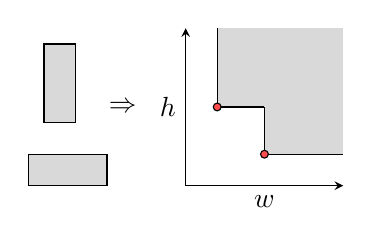
\begin{tikzpicture}[>=stealth,
    cpt/.style={draw,circle,inner sep=1pt},
    oldpt/.style={cpt,fill=blue!40},
    newpt/.style={cpt,fill=red!70}
  ]
  \begin{scope}
    \draw[fill=gray!30] (0.2,0.8) rectangle (0.6,1.8);
    \draw[fill=gray!30] (0,0) rectangle (1,0.4);
    \node at (1.2,1) {$\Rightarrow$};
  \end{scope}
  \begin{scope}[xshift=2cm]
    \draw[->] (0,0) -- (0,2) node[midway,left] {$h$};
    \draw[->] (0,0) -- (2,0) node[midway,below] {$w$};

    \draw[fill=gray!30,draw=none] (0.4,1) rectangle (2,2);
    \draw[fill=gray!30,draw=none] (1,0.4) rectangle (2,2);

    \draw (0.4,1) -- (1,1);
    \draw (0.4,1) -- (0.4,2);
    \draw (1,0.4) -- (1,1);
    \draw (1,0.4) -- (2,0.4);

    \node[newpt] at (0.4,1) {};
    \node[newpt] at (1,0.4) {};
  \end{scope}
\end{tikzpicture}
\end{center}
Step 2: Determine the shape fun. of the top-level floorplan\\
Choose minium bounding box ($w \times h$)
\begin{center}
\begin{tikzpicture}[>=stealth,
    cpt/.style={draw,circle,inner sep=1pt},
    oldpt/.style={cpt,fill=blue!40},
    newpt/.style={cpt,fill=red!70}
  ]
  \begin{scope}
    \draw[->] (0,0) -- (0,2) node[midway,left] {$h$};
    \draw[->] (0,0) -- (2,0) node[midway,below] (x) {$w$};
    \node at (1,-0.6) {a) vertical ($\uparrow$)};

    \node[oldpt] (a1) at (0.4,0.8) {};
    \node[oldpt] (a2) at (0.8,0.4) {};
    \node[oldpt] (b1) at (0.6,1.0) {};
    \node[oldpt] (b2) at (1.0,0.6) {};

    \draw[draw=none,fill=gray!20] (a1) rectangle (2,2);
    \draw[draw=none,fill=gray!20] (a2) rectangle (2,2);
    \draw (0.4,0.8) -- (0.8,0.8);
    \draw (0.8,0.4) -- (0.8,0.8);
    \draw (0.4,0.8) -- (0.4,2);
    \draw (0.8,0.4) -- (2,0.4);

    \draw[draw=none,fill=gray!60] (b1) rectangle (2,2);
    \draw[draw=none,fill=gray!60] (b2) rectangle (2,2);
    \draw (0.6,1.0) -- (1.0,1.0);
    \draw (1.0,0.6) -- (1.0,1.0);
    \draw (0.6,1.0) -- (0.6,2);
    \draw (1.0,0.6) -- (2,0.6);

    \node[oldpt] at (a1) {};
    \node[oldpt] at (a2) {};
    \node[oldpt] at (b1) {};
    \node[oldpt] at (b2) {};

    \node[newpt] (c1) at (0.6,1.8) {};
    \node[newpt] (c2) at (0.8,1.4) {};
    \node[newpt] (c3) at (1.0,1.0) {};

    \draw[draw=none,fill=white] (c1) rectangle (2,2);
    \draw[draw=none,fill=white] (c2) rectangle (2,2);
    \draw[draw=none,fill=white] (c3) rectangle (2,2);
    \draw[draw=none,pattern=north east lines] (c1) rectangle (2,2);
    \draw[draw=none,pattern=north east lines] (c2) rectangle (2,2);
    \draw[draw=none,pattern=north east lines] (c3) rectangle (2,2);
    \draw (0.6,2) -- (0.6,1.8)
      -- (0.8,1.8) -- (0.8,1.4)
      -- (1,1.4) -- (1,1) -- (2,1);

    \node[newpt] (c1) at (0.6,1.8) {};
    \node[newpt] (c2) at (0.8,1.4) {};
    \node[newpt] (c3) at (1.0,1.0) {};
  \end{scope}
  \begin{scope}[xshift=3.5cm]
    \draw[->] (0,0) -- (0,2) node[midway,left] {$h$};
    \draw[->] (0,0) -- (2,0) node[midway,below] {$w$};
    \node at (1,-0.6) {b) horizontal ($\rightarrow$)};

    \node[oldpt] (a1) at (0.4,0.8) {};
    \node[oldpt] (a2) at (0.8,0.4) {};
    \node[oldpt] (b1) at (0.6,1.0) {};
    \node[oldpt] (b2) at (1.0,0.6) {};

    \draw[draw=none,fill=gray!20] (a1) rectangle (2,2);
    \draw[draw=none,fill=gray!20] (a2) rectangle (2,2);
    \draw (0.4,0.8) -- (0.8,0.8);
    \draw (0.8,0.4) -- (0.8,0.8);
    \draw (0.4,0.8) -- (0.4,2);
    \draw (0.8,0.4) -- (2,0.4);

    \draw[draw=none,fill=gray!60] (b1) rectangle (2,2);
    \draw[draw=none,fill=gray!60] (b2) rectangle (2,2);
    \draw (0.6,1.0) -- (1.0,1.0);
    \draw (1.0,0.6) -- (1.0,1.0);
    \draw (0.6,1.0) -- (0.6,2);
    \draw (1.0,0.6) -- (2,0.6);

    \node[oldpt] at (a1) {};
    \node[oldpt] at (a2) {};
    \node[oldpt] at (b1) {};
    \node[oldpt] at (b2) {};

    \node[newpt] (c1) at (1.8,0.6) {};
    \node[newpt] (c2) at (1.4,0.8) {};
    \node[newpt] (c3) at (1.0,1.0) {};

    \draw[draw=none,fill=white] (c1) rectangle (2,2);
    \draw[draw=none,fill=white] (c2) rectangle (2,2);
    \draw[draw=none,fill=white] (c3) rectangle (2,2);
    \draw[draw=none,pattern=north east lines] (c1) rectangle (2,2);
    \draw[draw=none,pattern=north east lines] (c2) rectangle (2,2);
    \draw[draw=none,pattern=north east lines] (c3) rectangle (2,2);
    \draw (2,0.6) -- (1.8,0.6)
      -- (1.8,0.8) -- (1.4,0.8)
      -- (1.4,1) -- (1,1) -- (1,2);

    \node[newpt] (c1) at (1.8,0.6) {};
    \node[newpt] (c2) at (1.4,0.8) {};
    \node[newpt] (c3) at (1.0,1.0) {};
  \end{scope}
\end{tikzpicture}
\end{center}
Step 3: Find individual block's dimensions and locations

\describe{Cluster Growth}
\begin{itemize}
  \item Iteratively add blocks to the cluster until all are assigned
  \item Only the different orientations of the blocks are taken into account
  \item Linear ordering to minimize total wire length
\end{itemize}
\alert{Continue..?}
